\Exhibit{ZamanaVideo}{
    Скриншоты и транскрипт сюжета с фокусом на методологию Школы Граня
    и их учебные наборы на KTRK\WithTr%
}

Это скриншоты и транскрипт сюжета, вышедшего в утренней программе `Zamana',
о развивающем центре для детей в Бишкеке, столице Киргизии,
с фокусом на методологию Сергея Граня и учебные наборы,
которые школа производит.

Достоверность видео подтверждается его присутствием в группе программы в Facebook.

Достоверность программы также дополнительно подтверждается на сайте телеканала \ExhibitRef{ZamanaUtrk}.

На 0:54 показан учебник Школы Граня по работе с огнём:

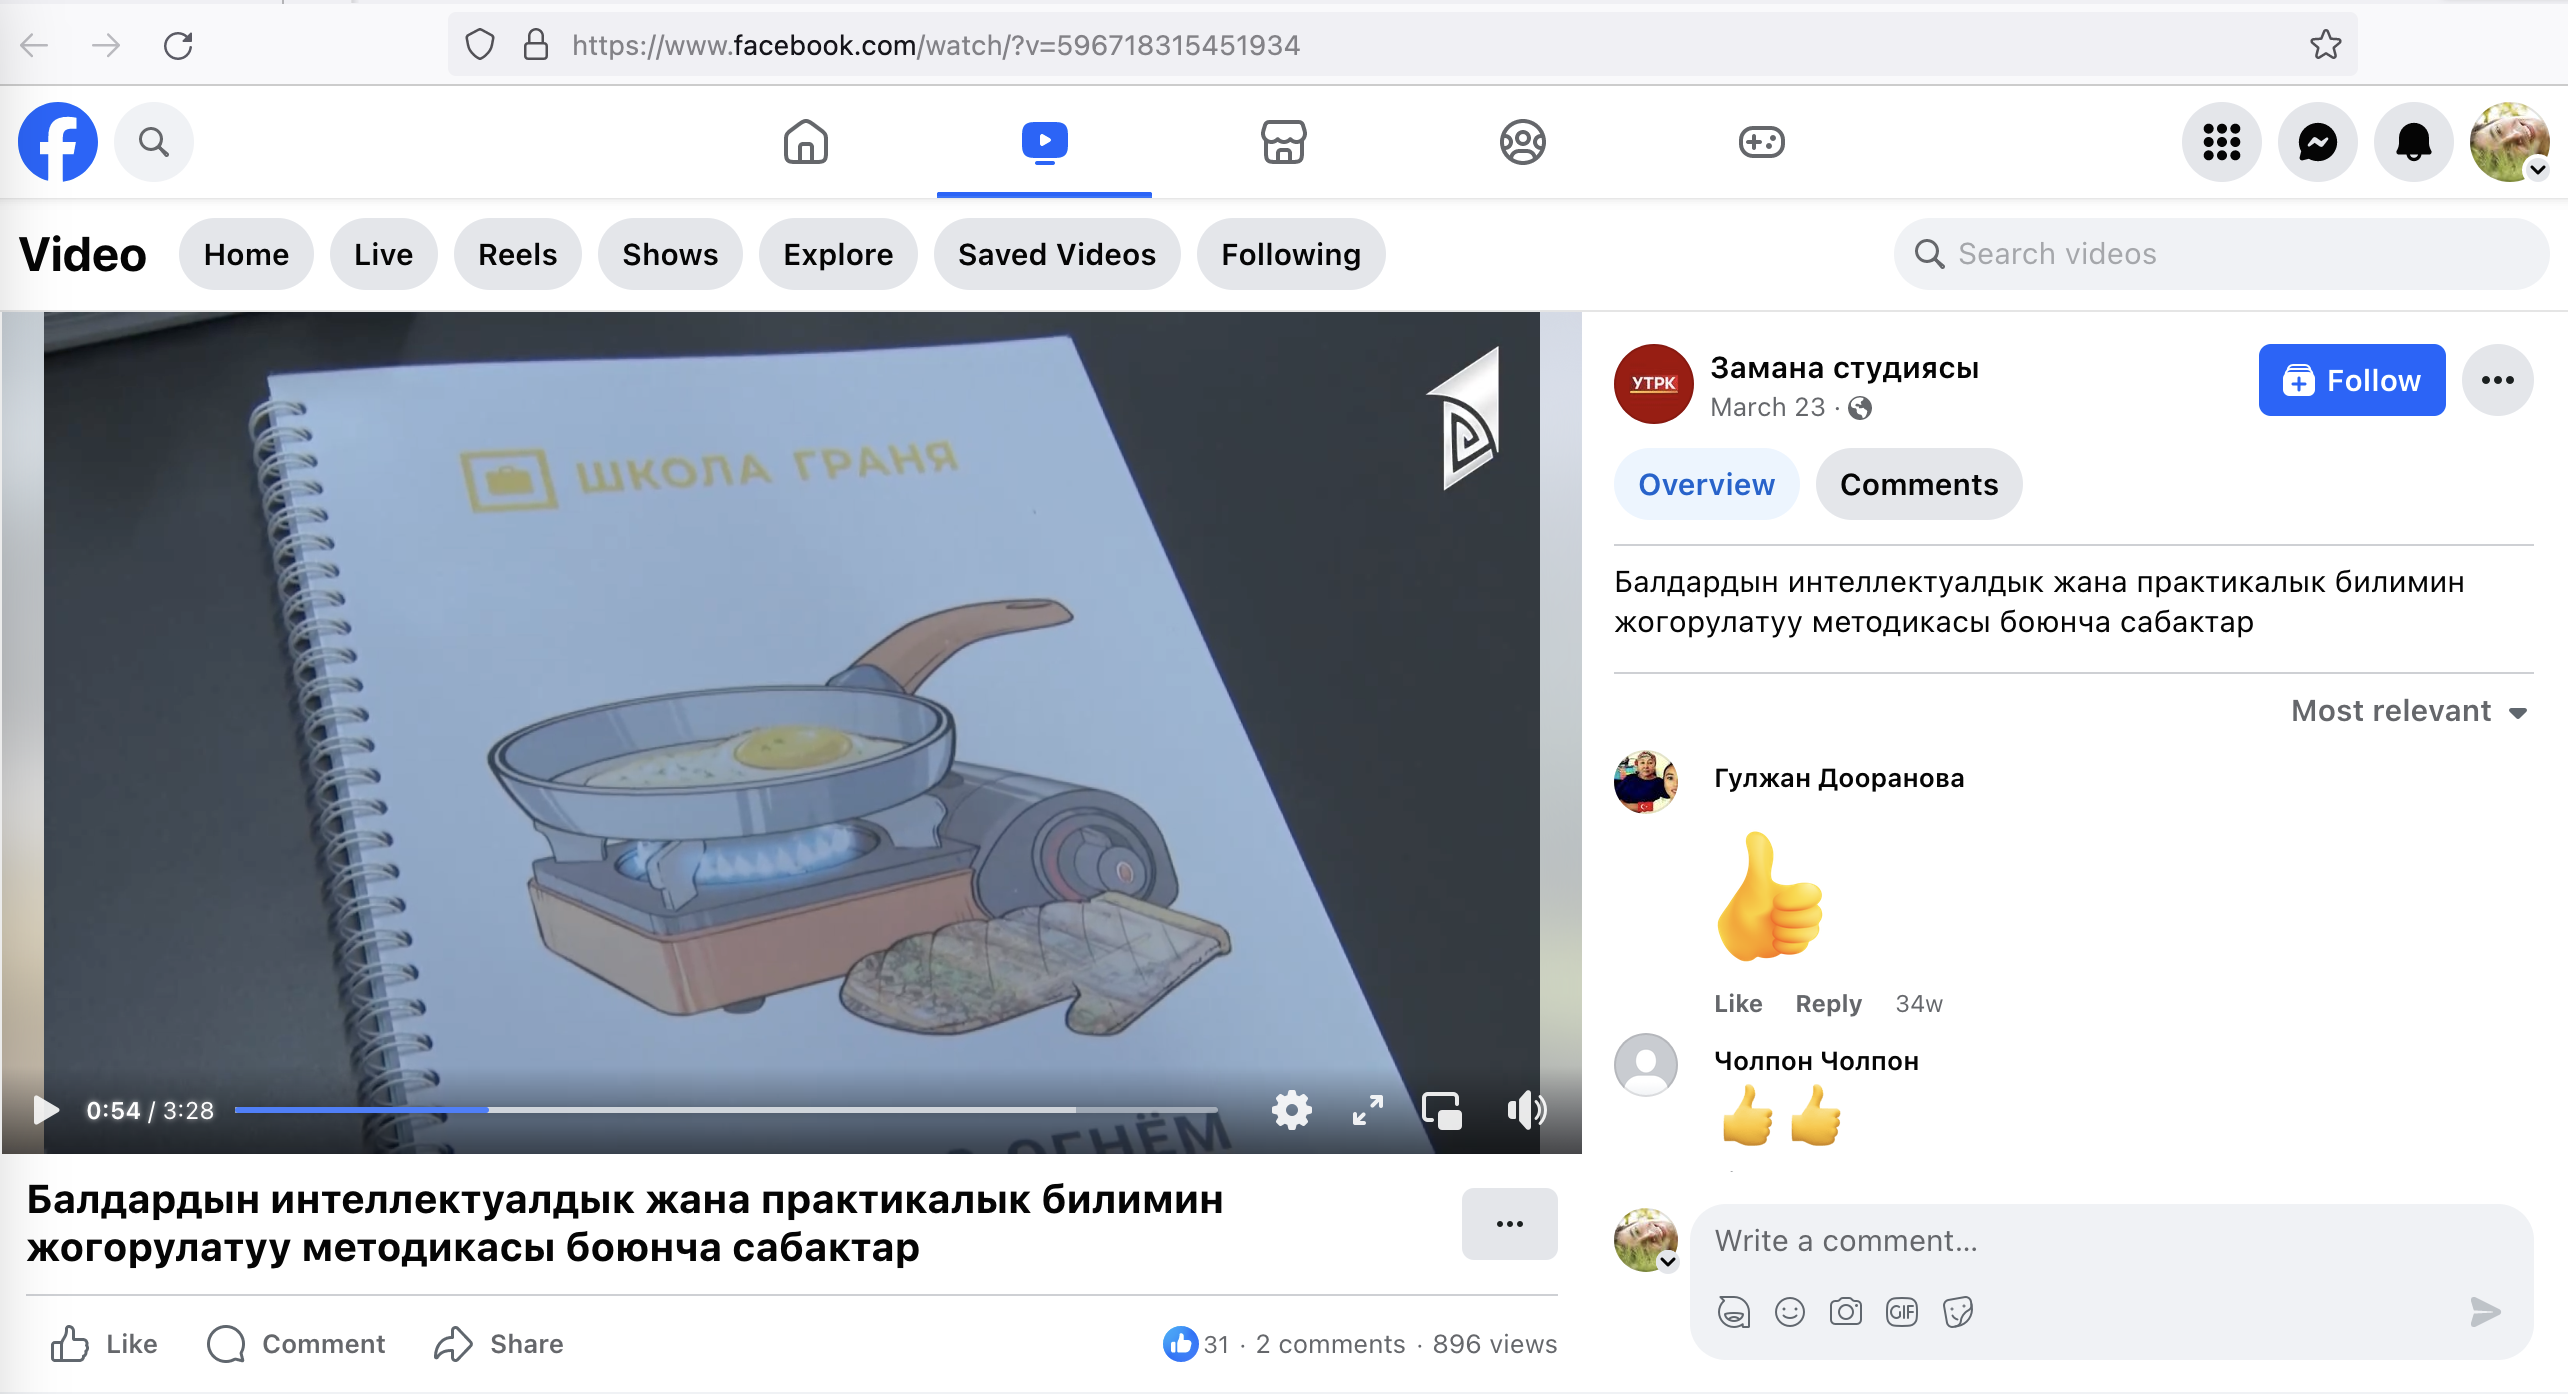
\includegraphics[width=\textwidth]{0_54_book-fire}

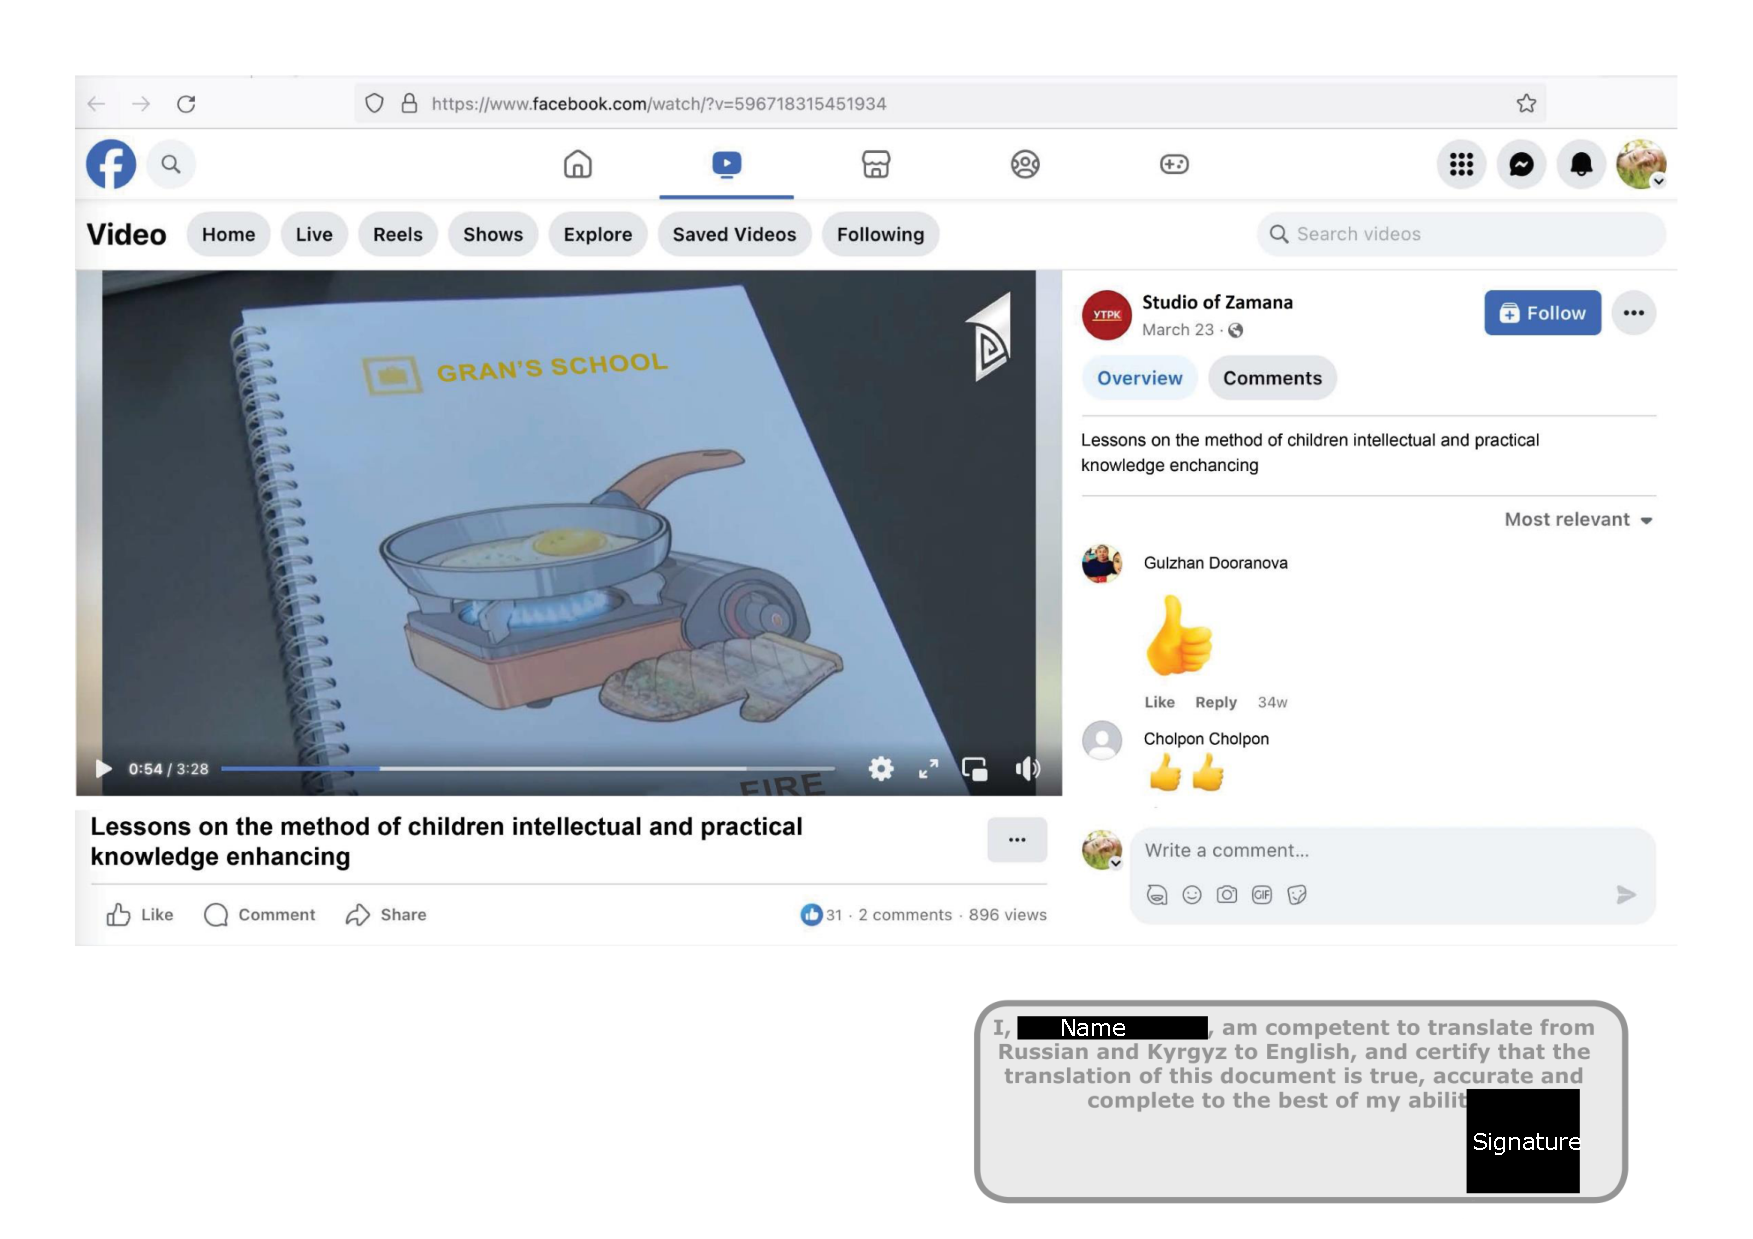
\includepdf[pages=-,angle=90]{0_54_book-fire_en_public}

Этот скриншот также показывает, что у группы 78 тысяч подписчиков.
Он также показывает ссылку на сайт канала, что подтверждает подлинность:

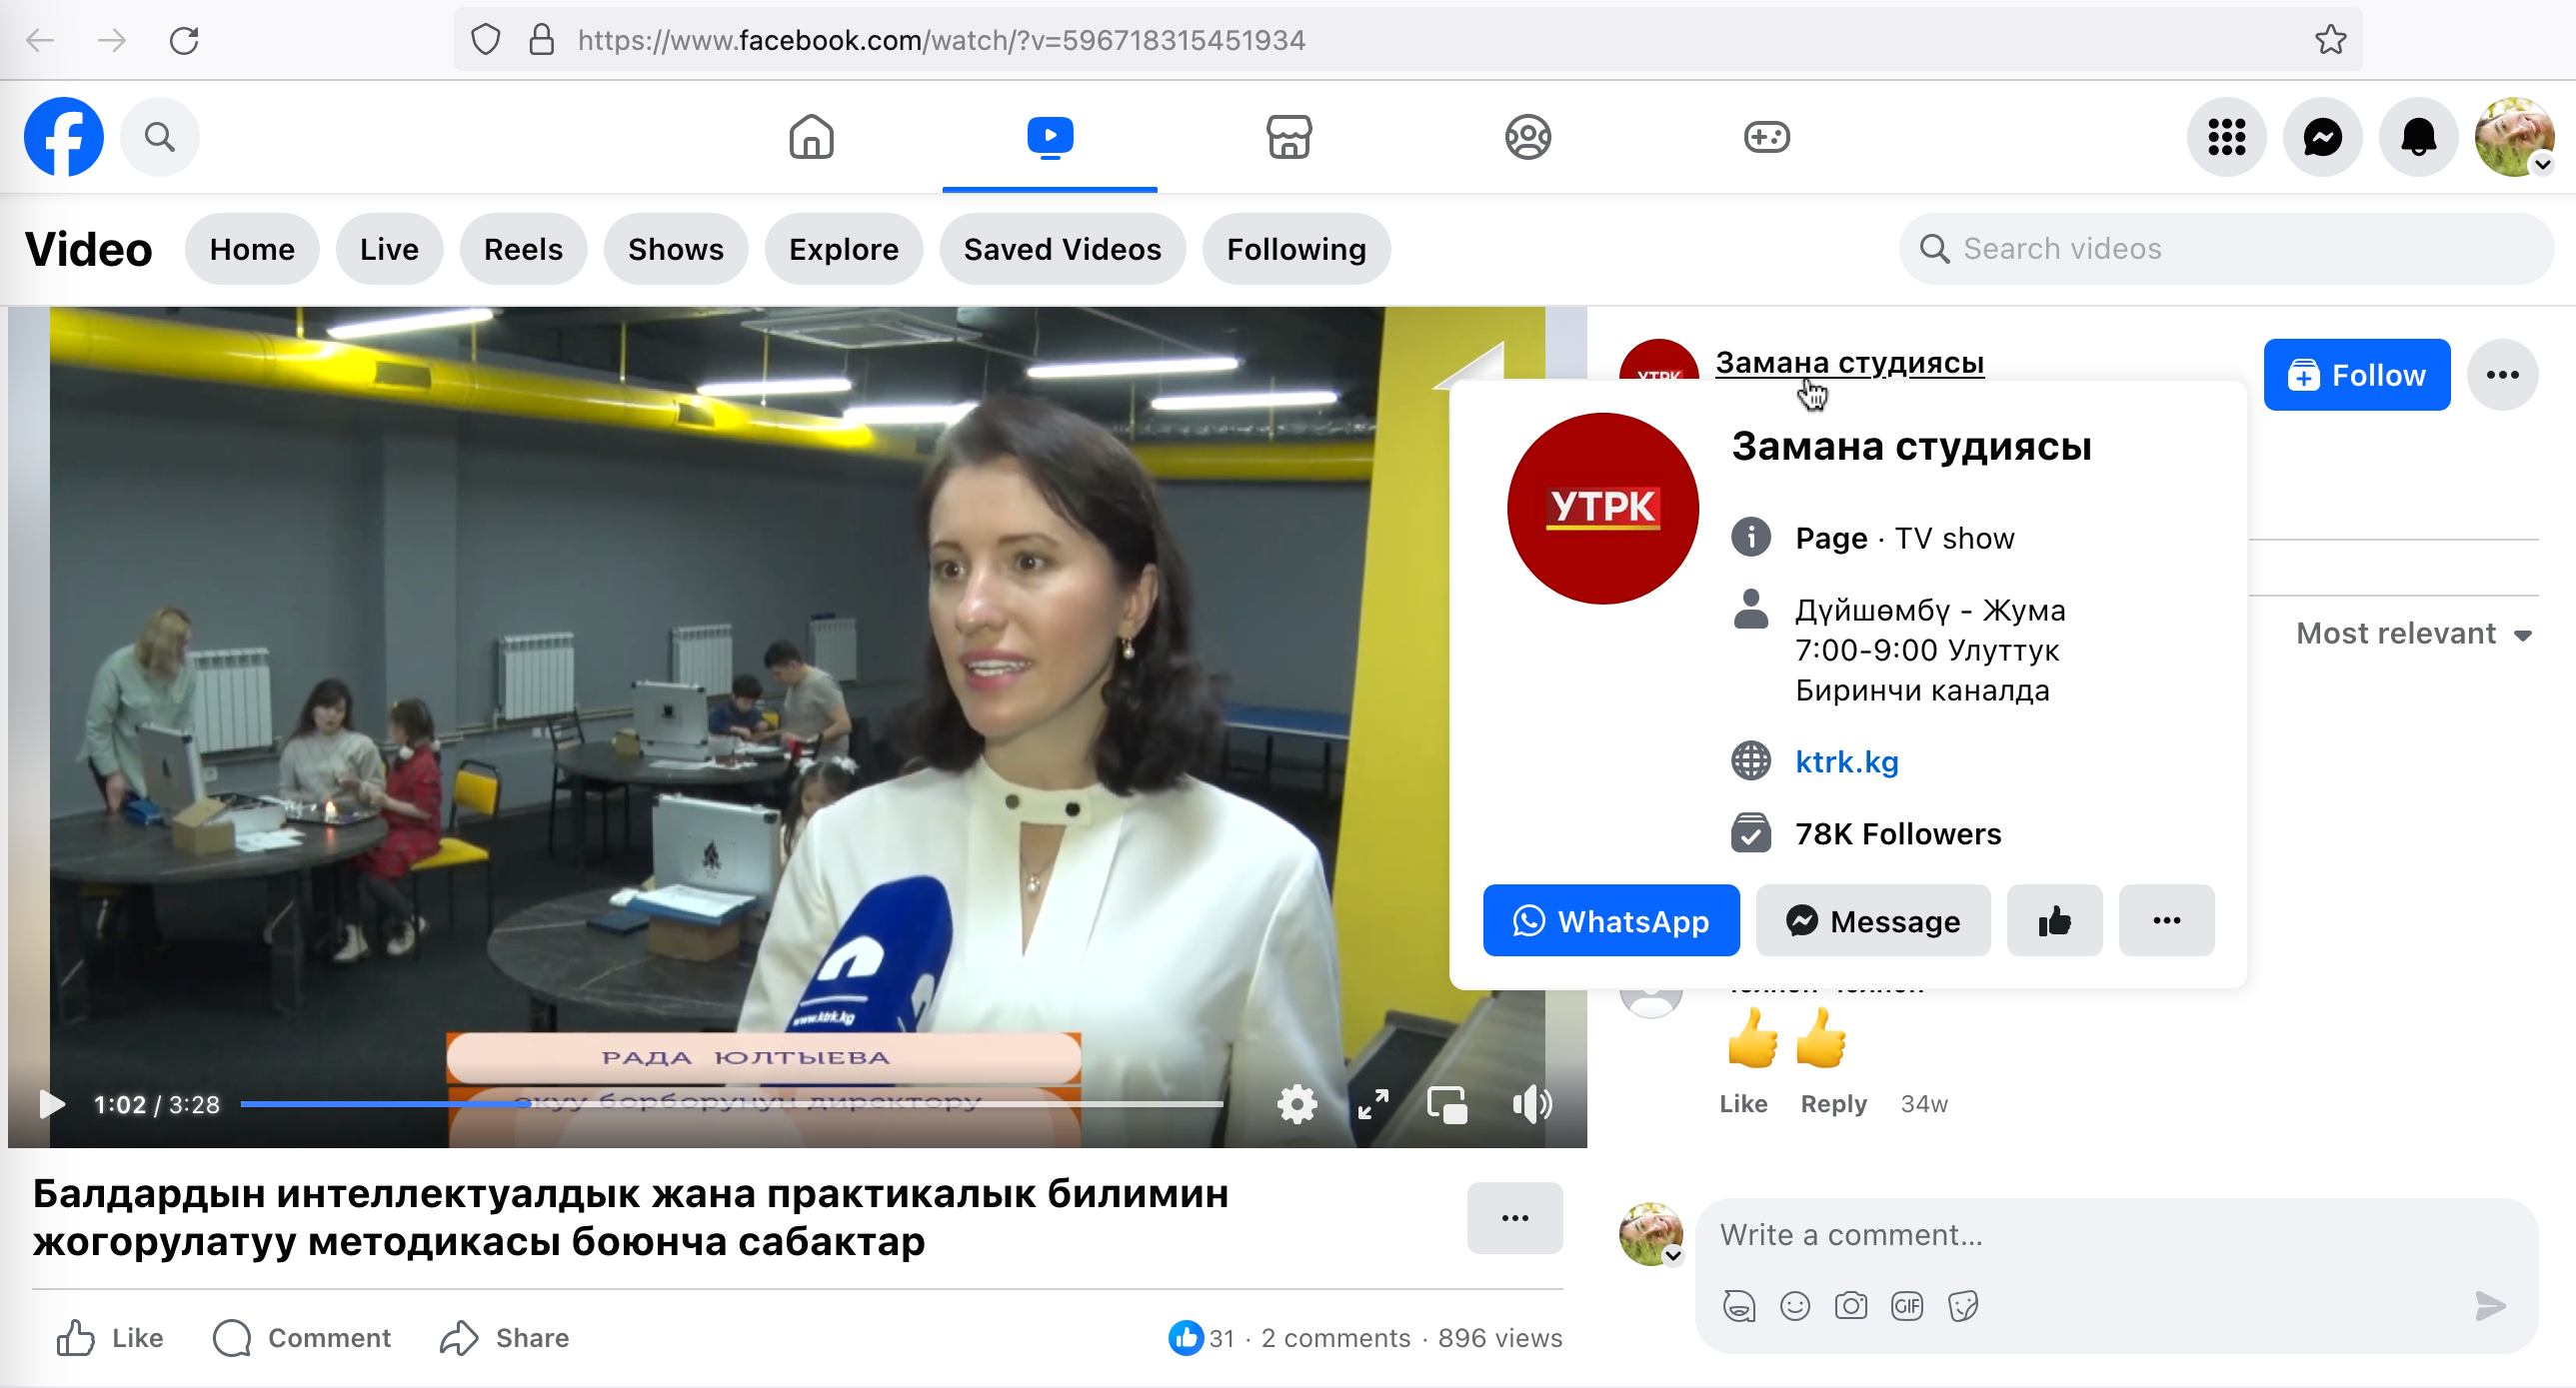
\includegraphics[width=\textwidth]{1_02_rada-stats}

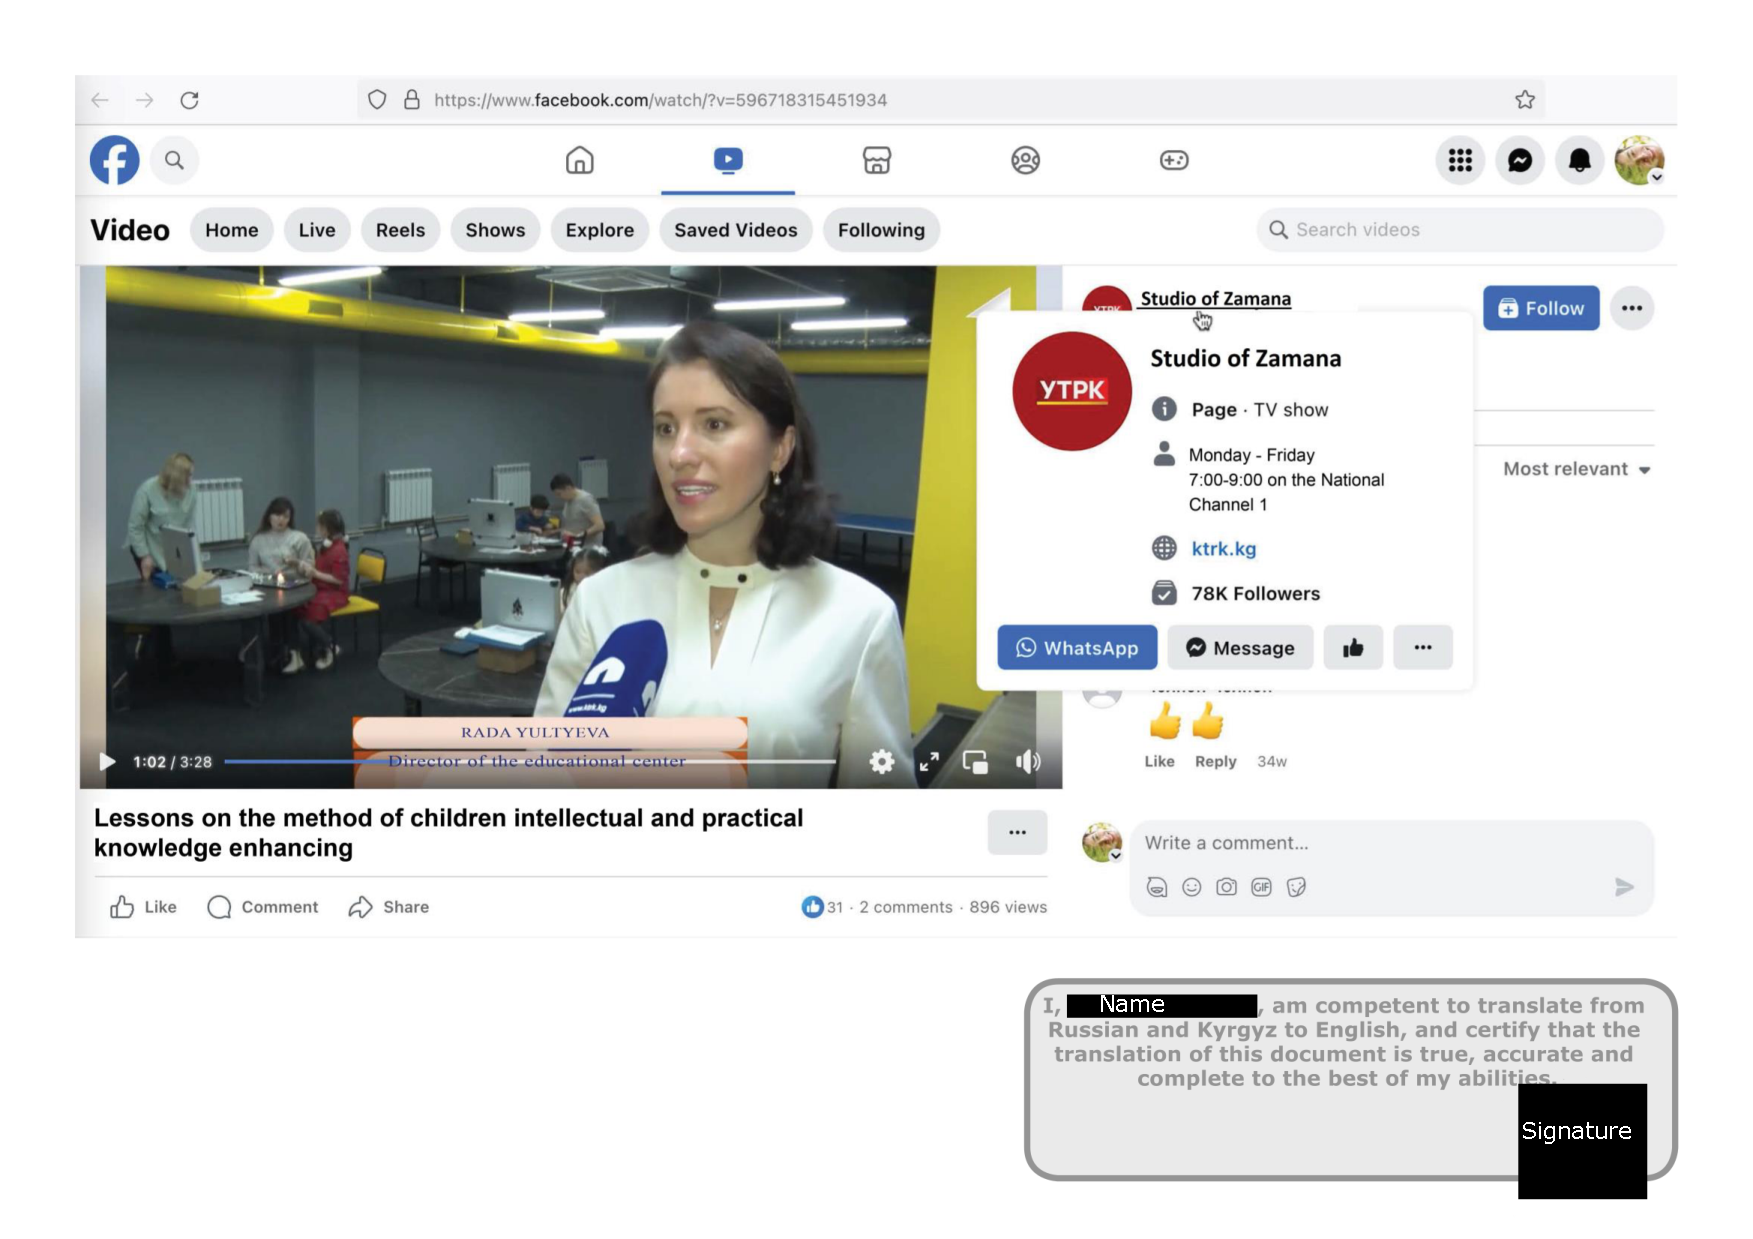
\includepdf[pages=-,angle=90]{1_02_rada-stats_en_public}

На 2:30 виден микрофон с адресом `ktrk.kg', что дополнительно подтверждает подлинность:

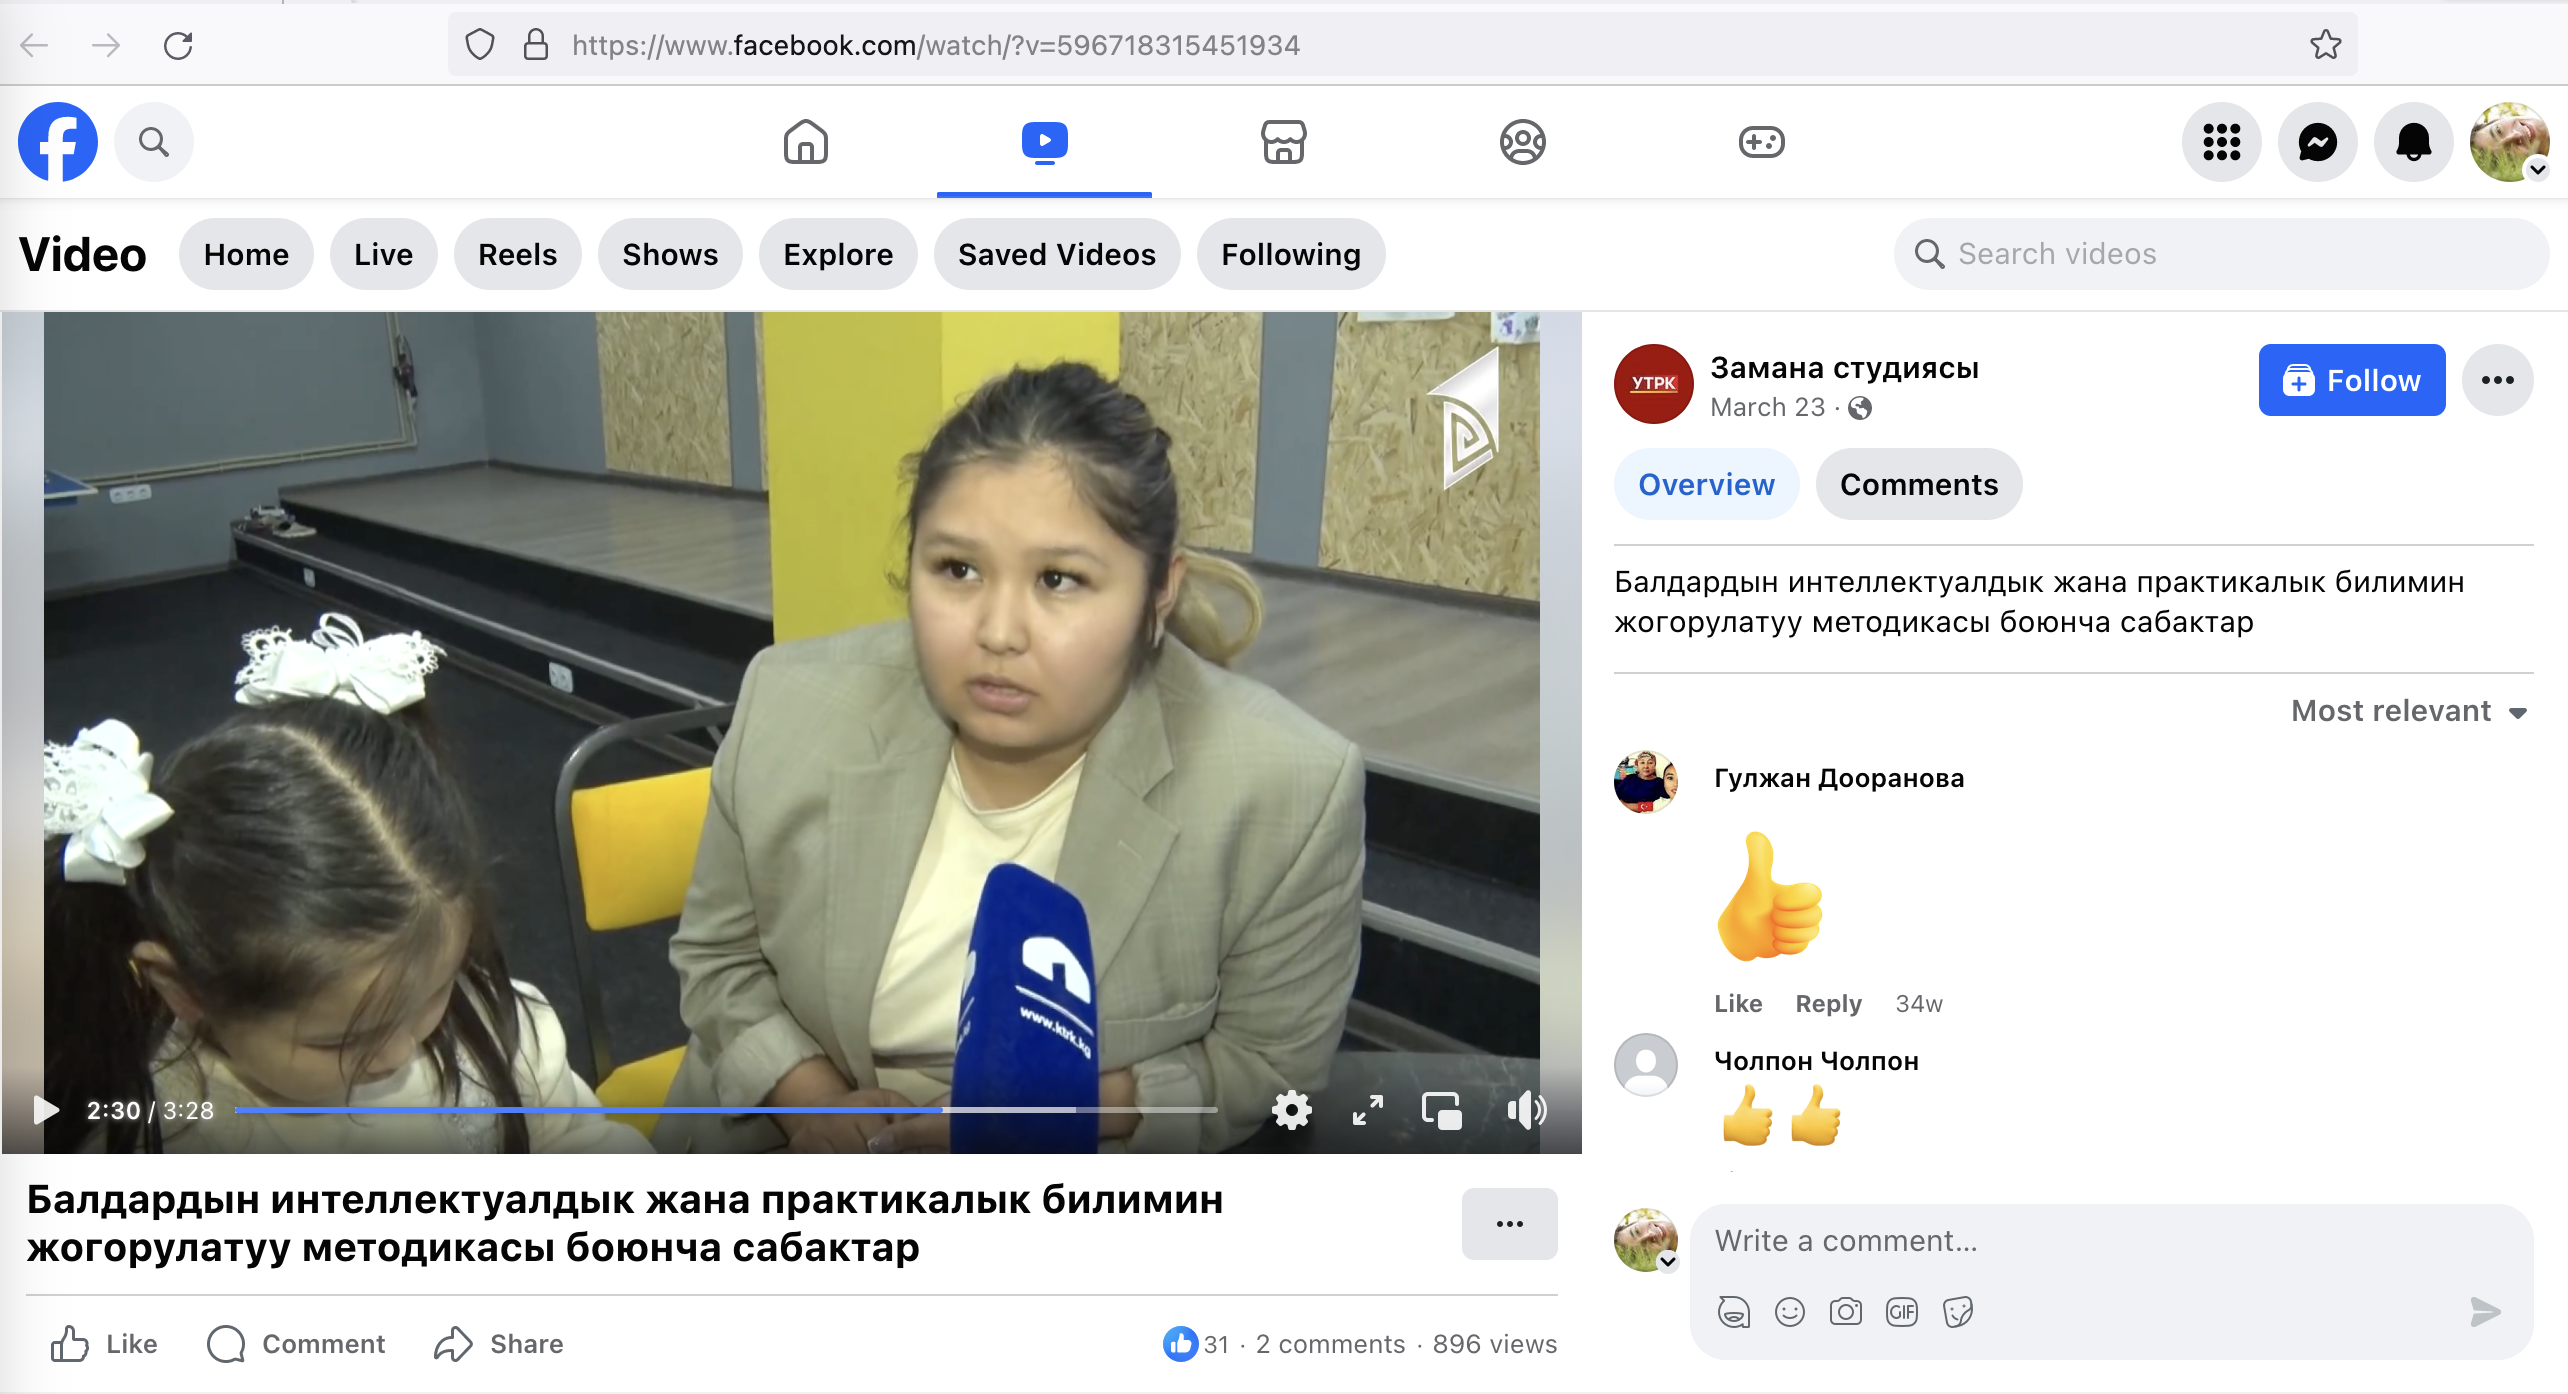
\includegraphics[width=\textwidth]{2_30_girls}

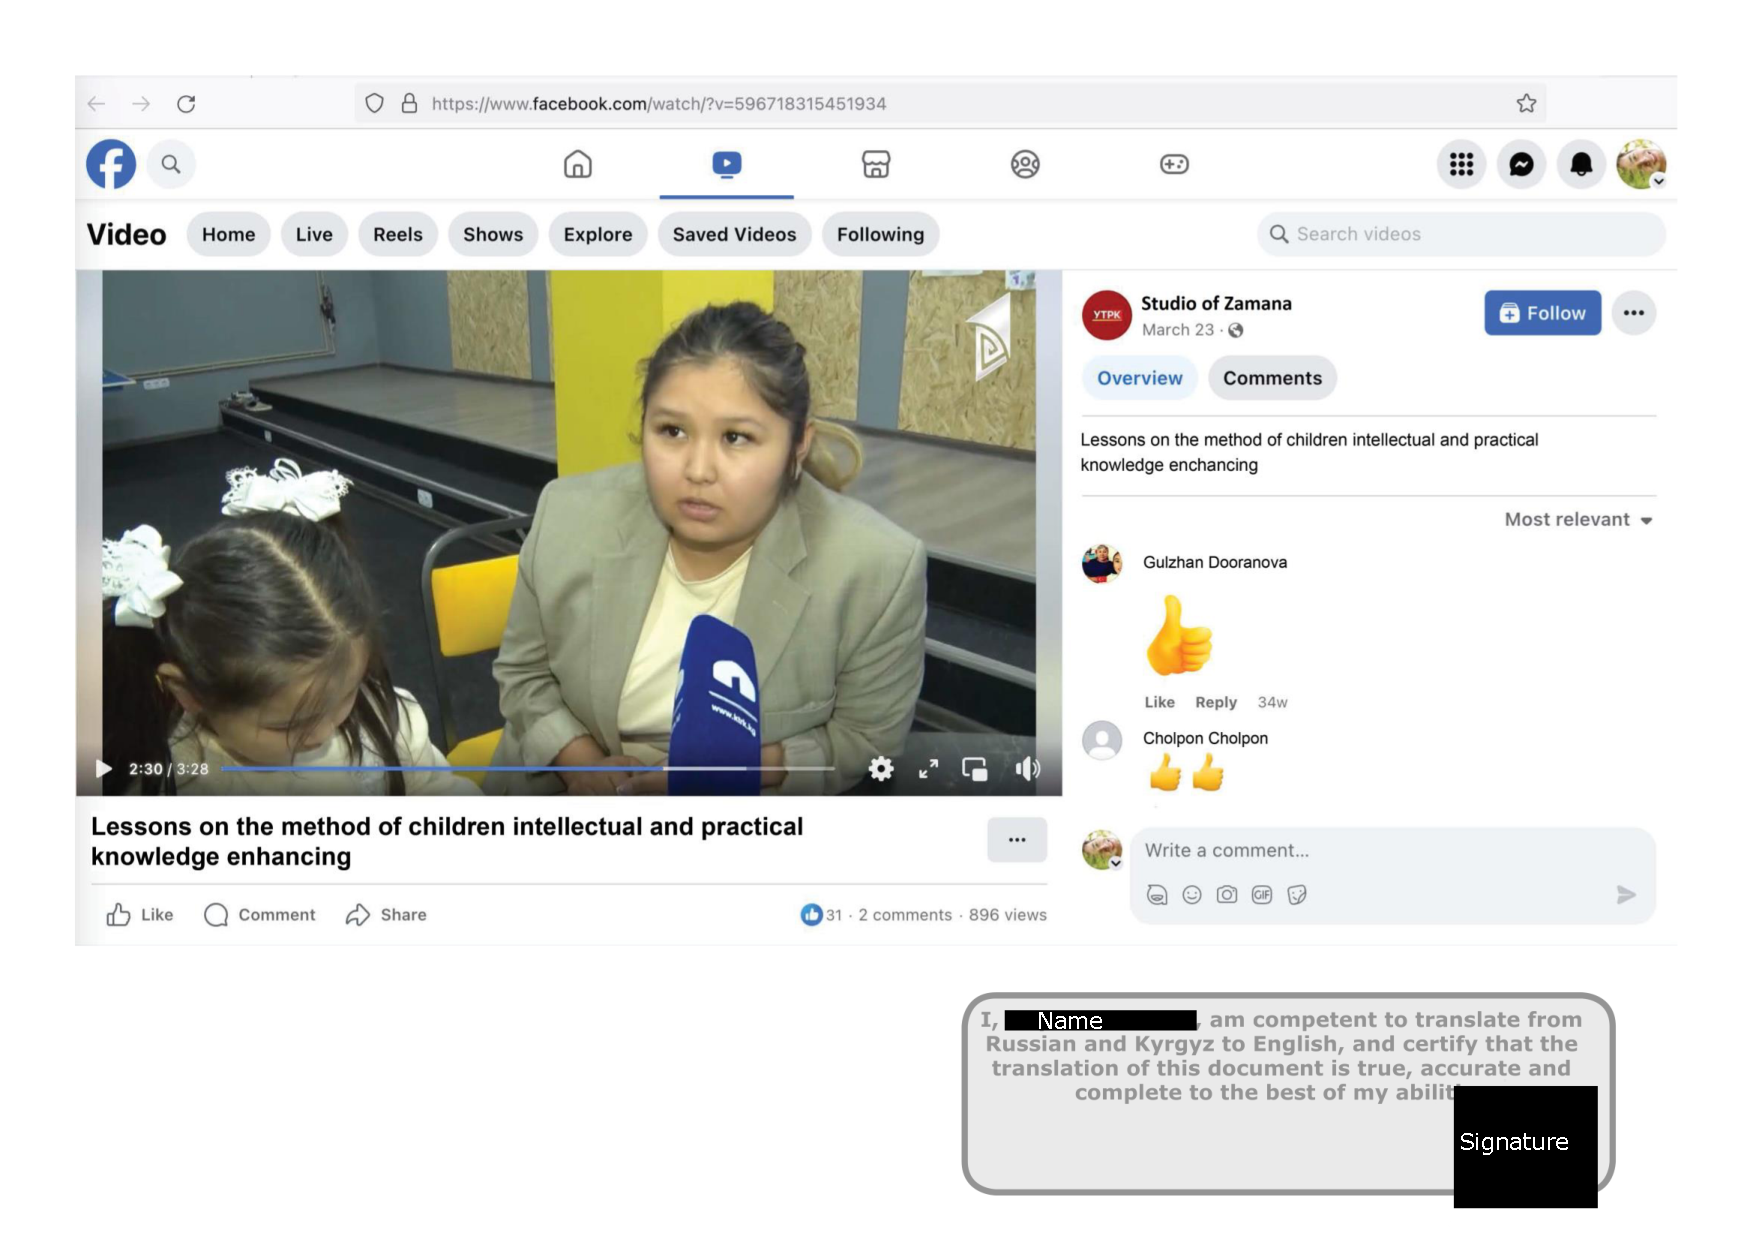
\includepdf[pages=-,angle=90]{2_30_girls_en_public}

На 3:16 виден другой учебник Школы Граня -- по работе с глиной:

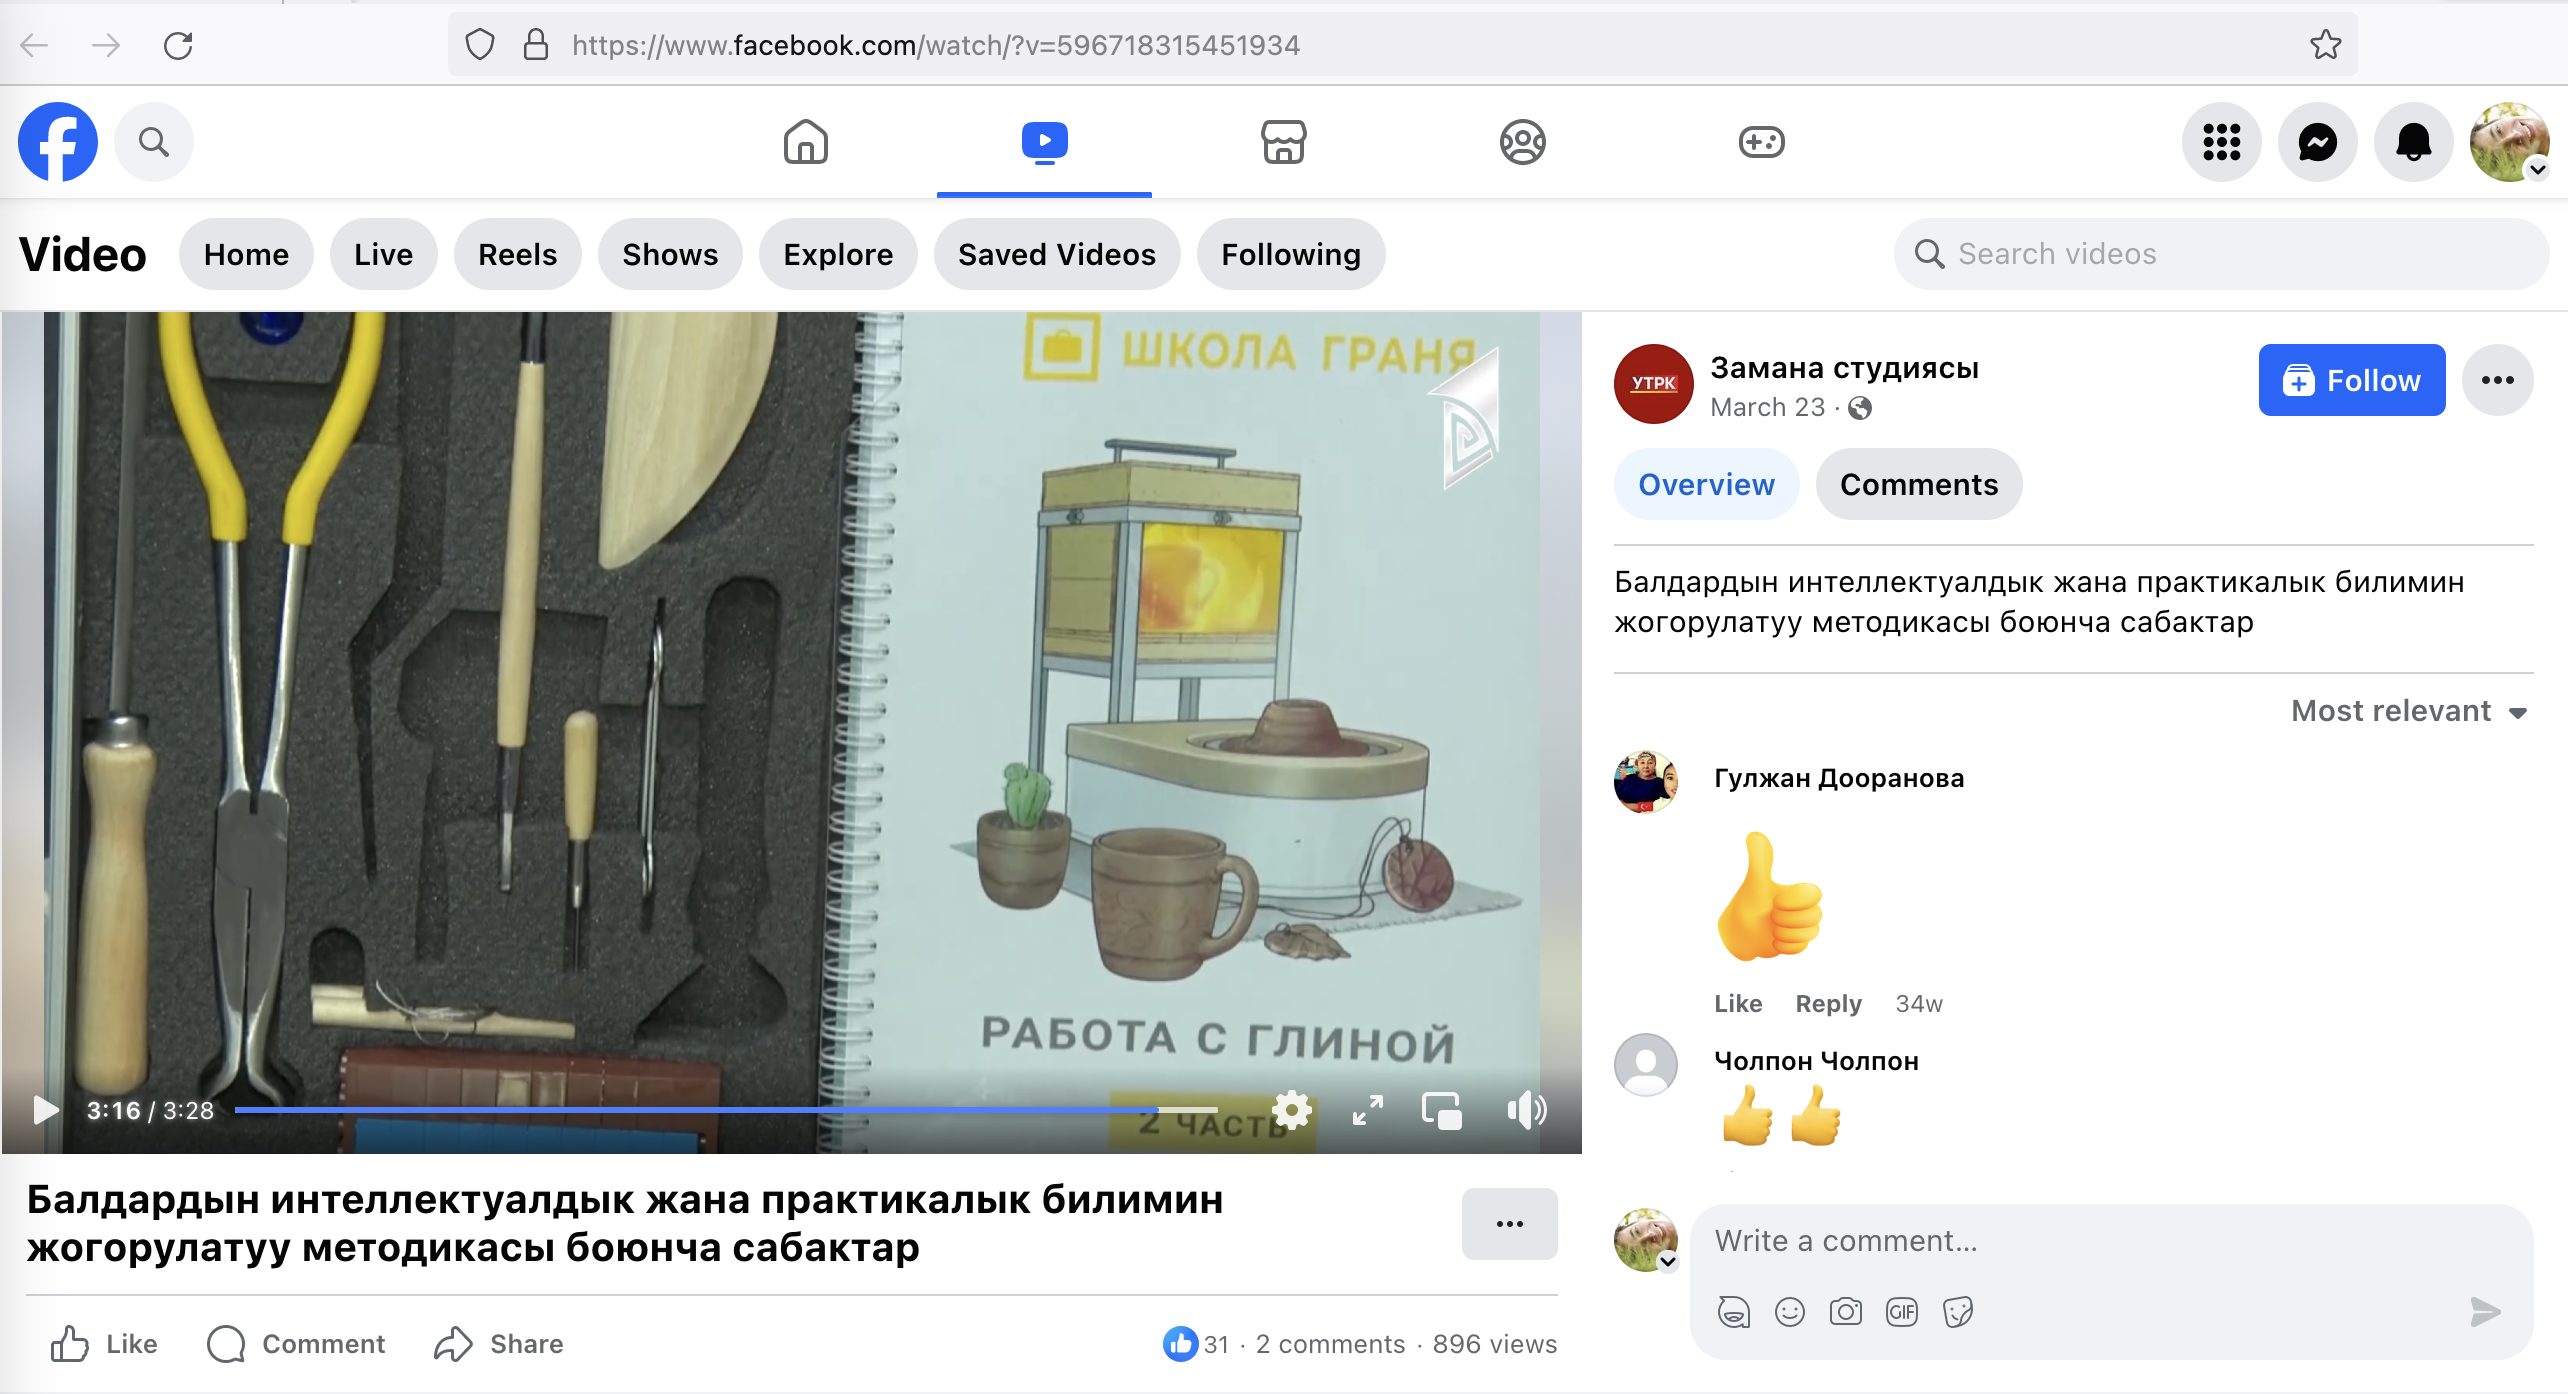
\includegraphics[width=\textwidth]{3_16_book-clay}

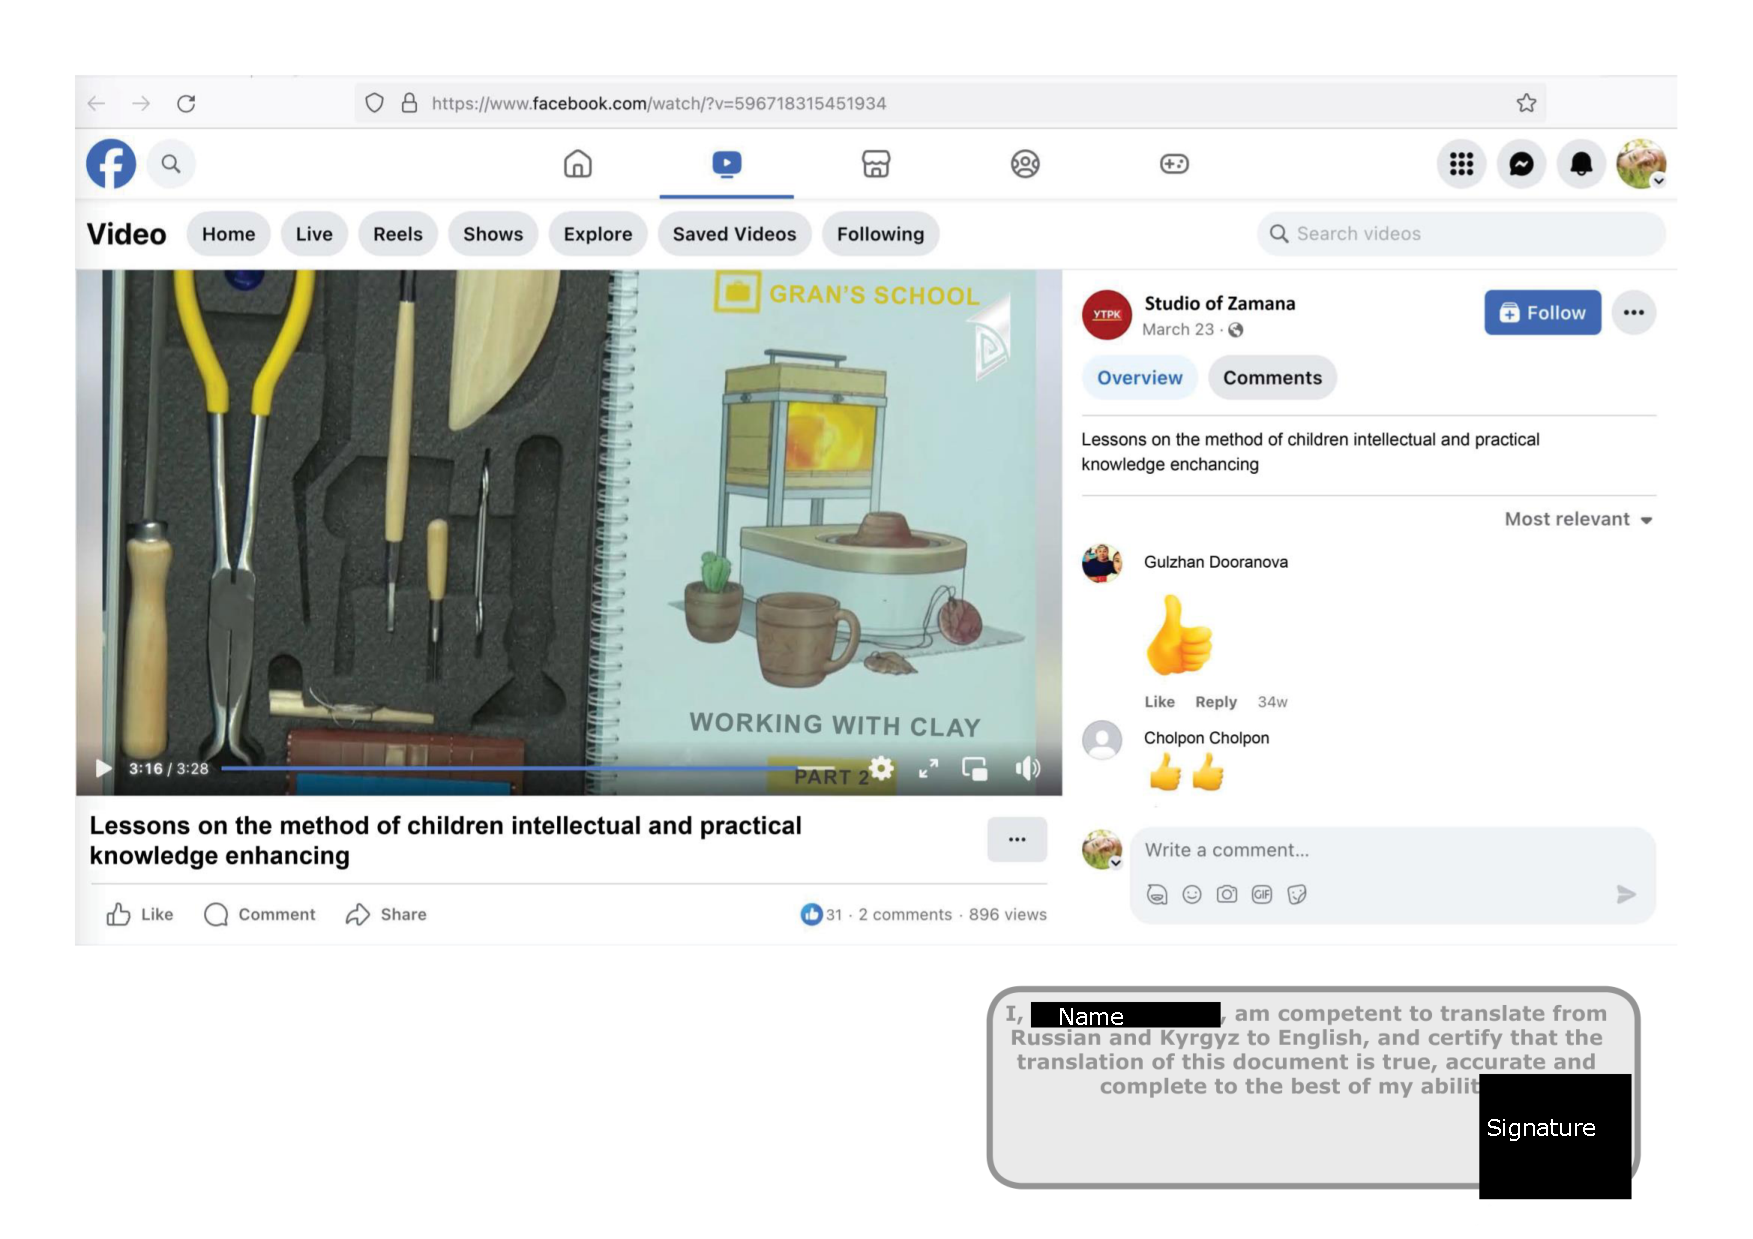
\includepdf[pages=-,angle=90]{3_16_book-clay_en_public}

На 3:28 -- три ребёнка:

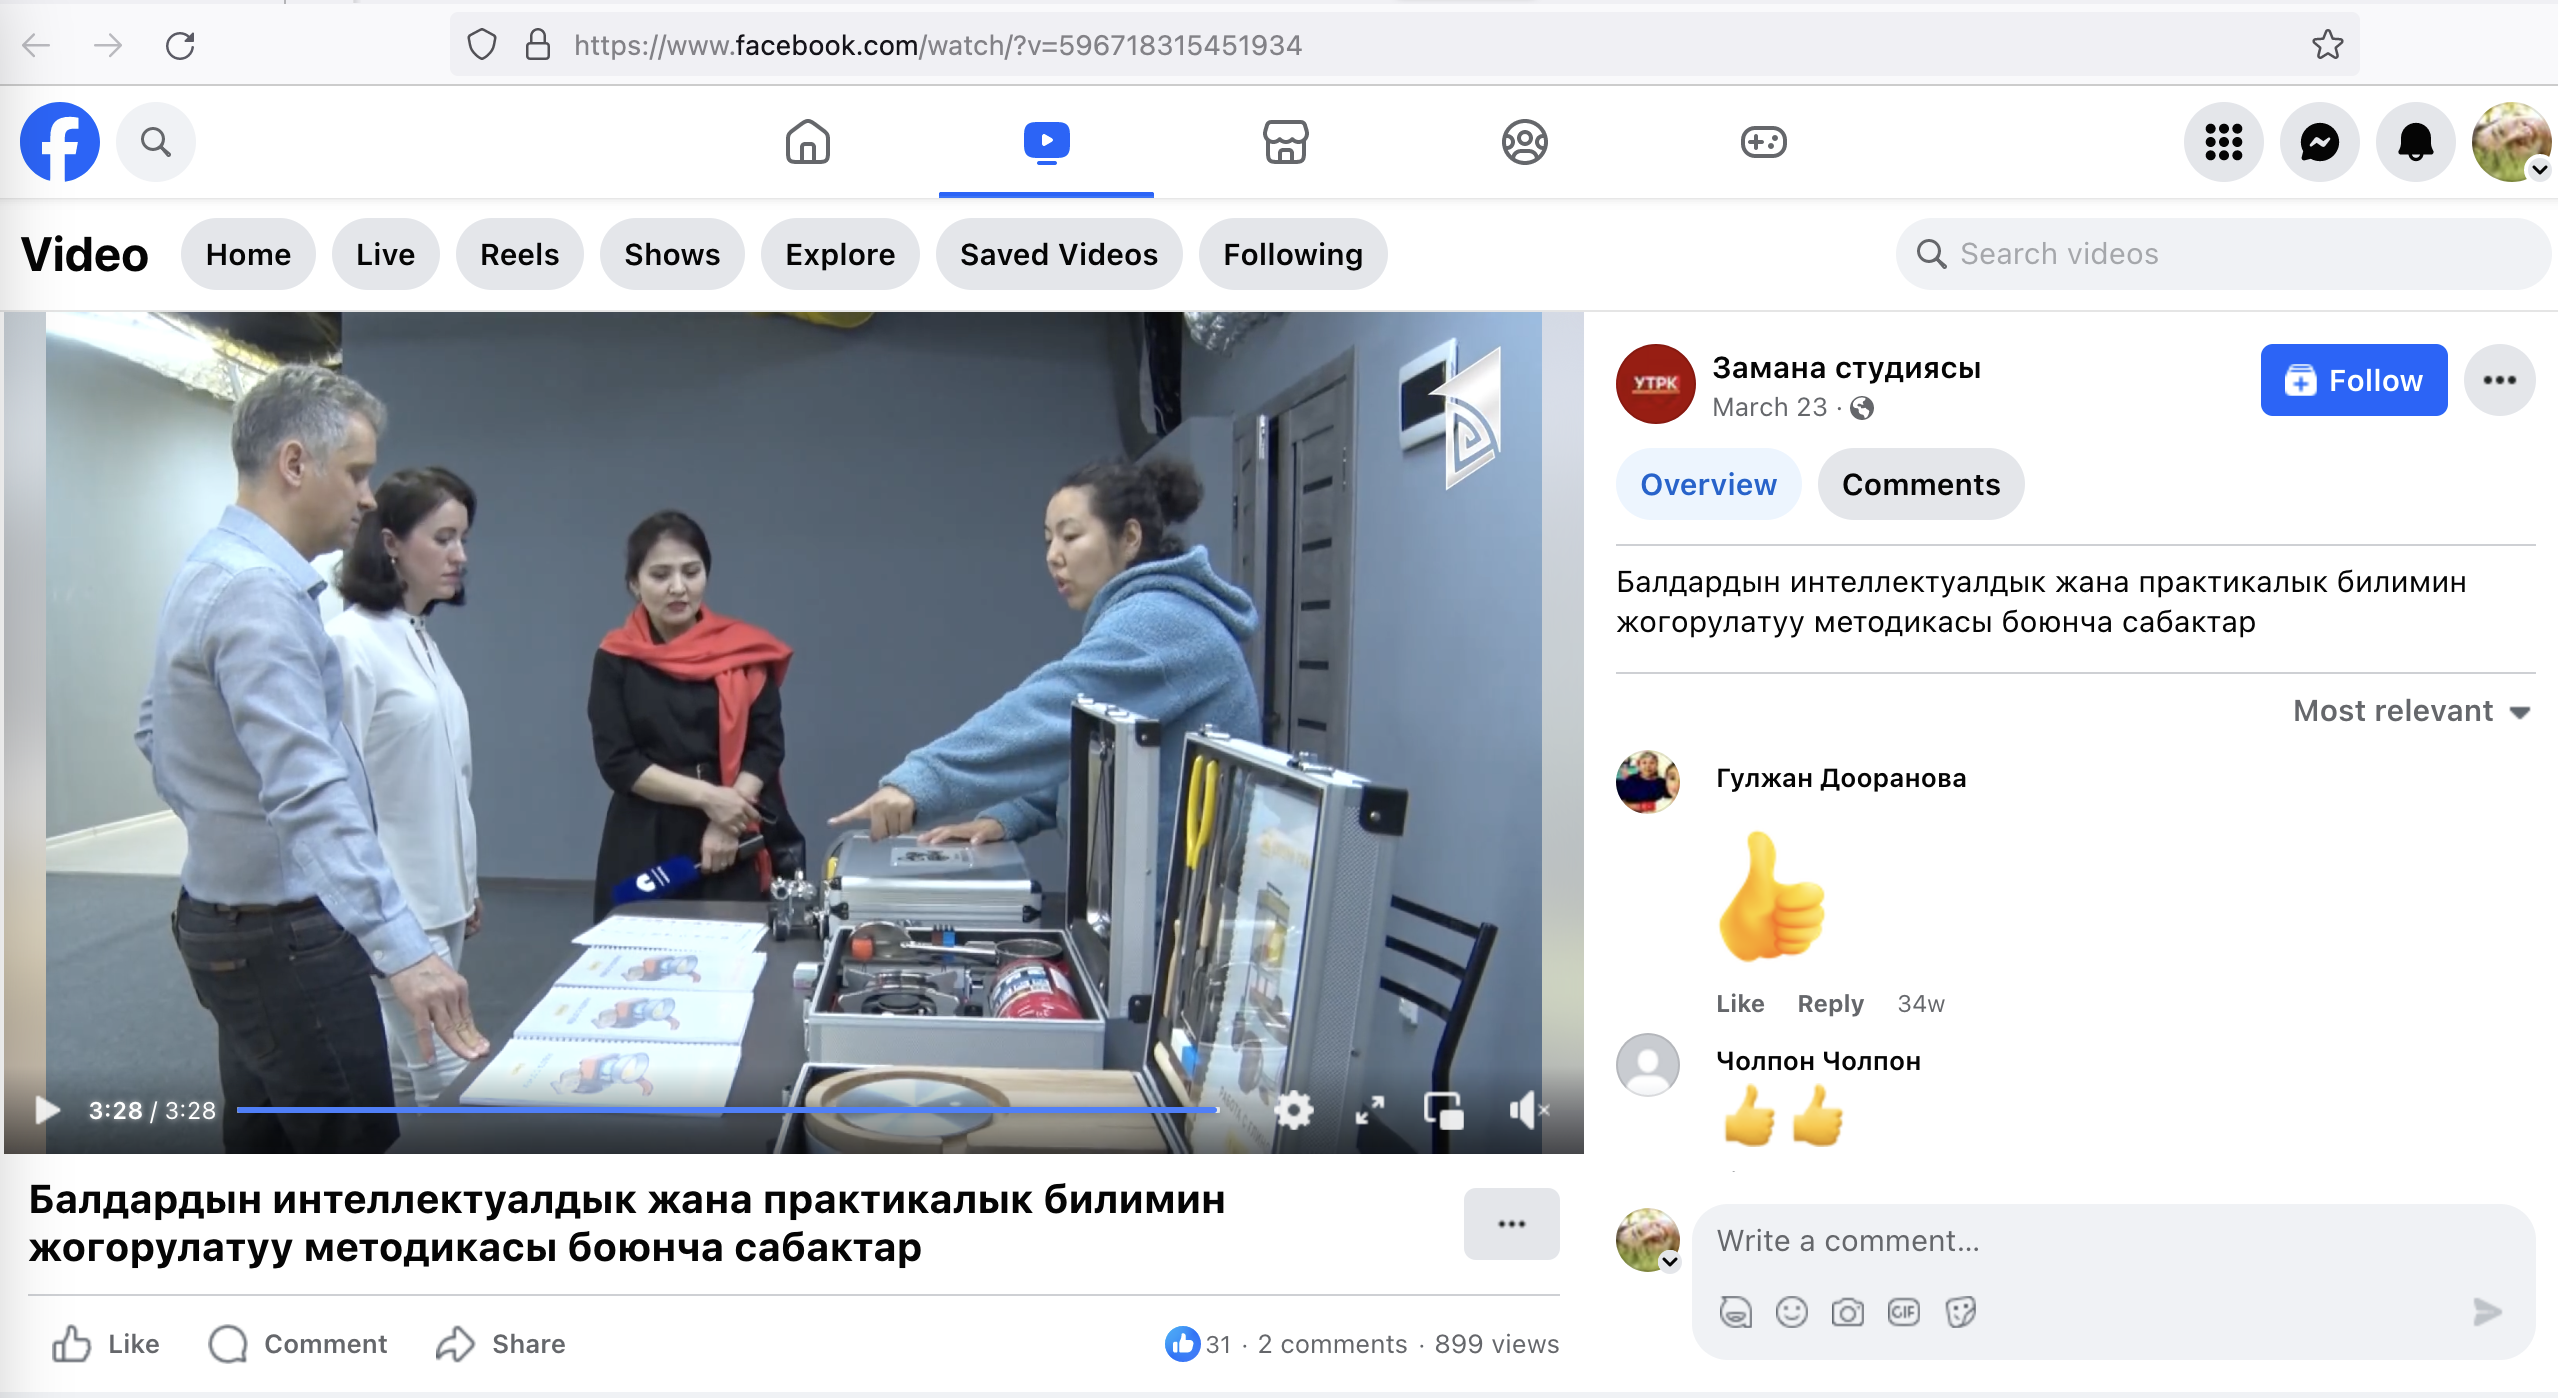
\includegraphics[width=\textwidth]{3_28_stand}

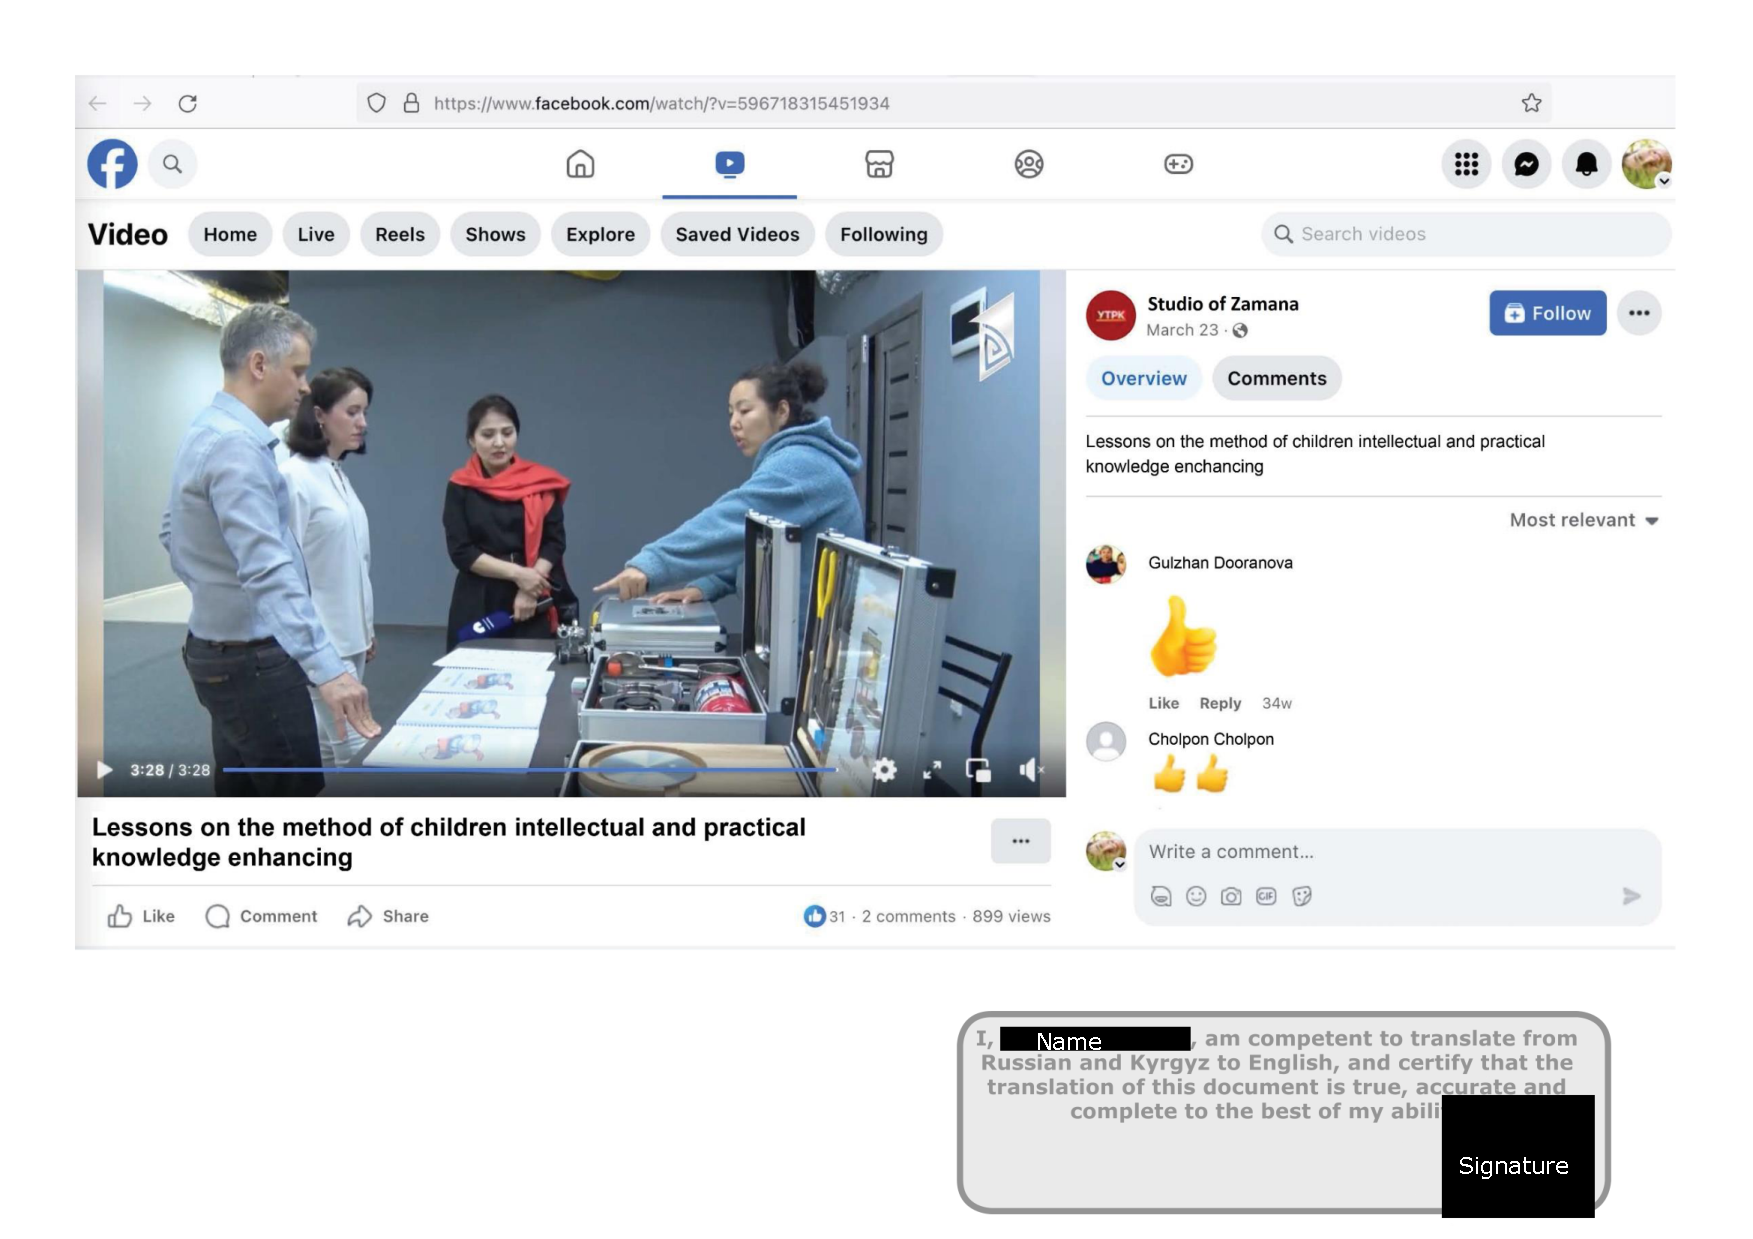
\includepdf[pages=-,angle=90]{3_28_stand_en_public}

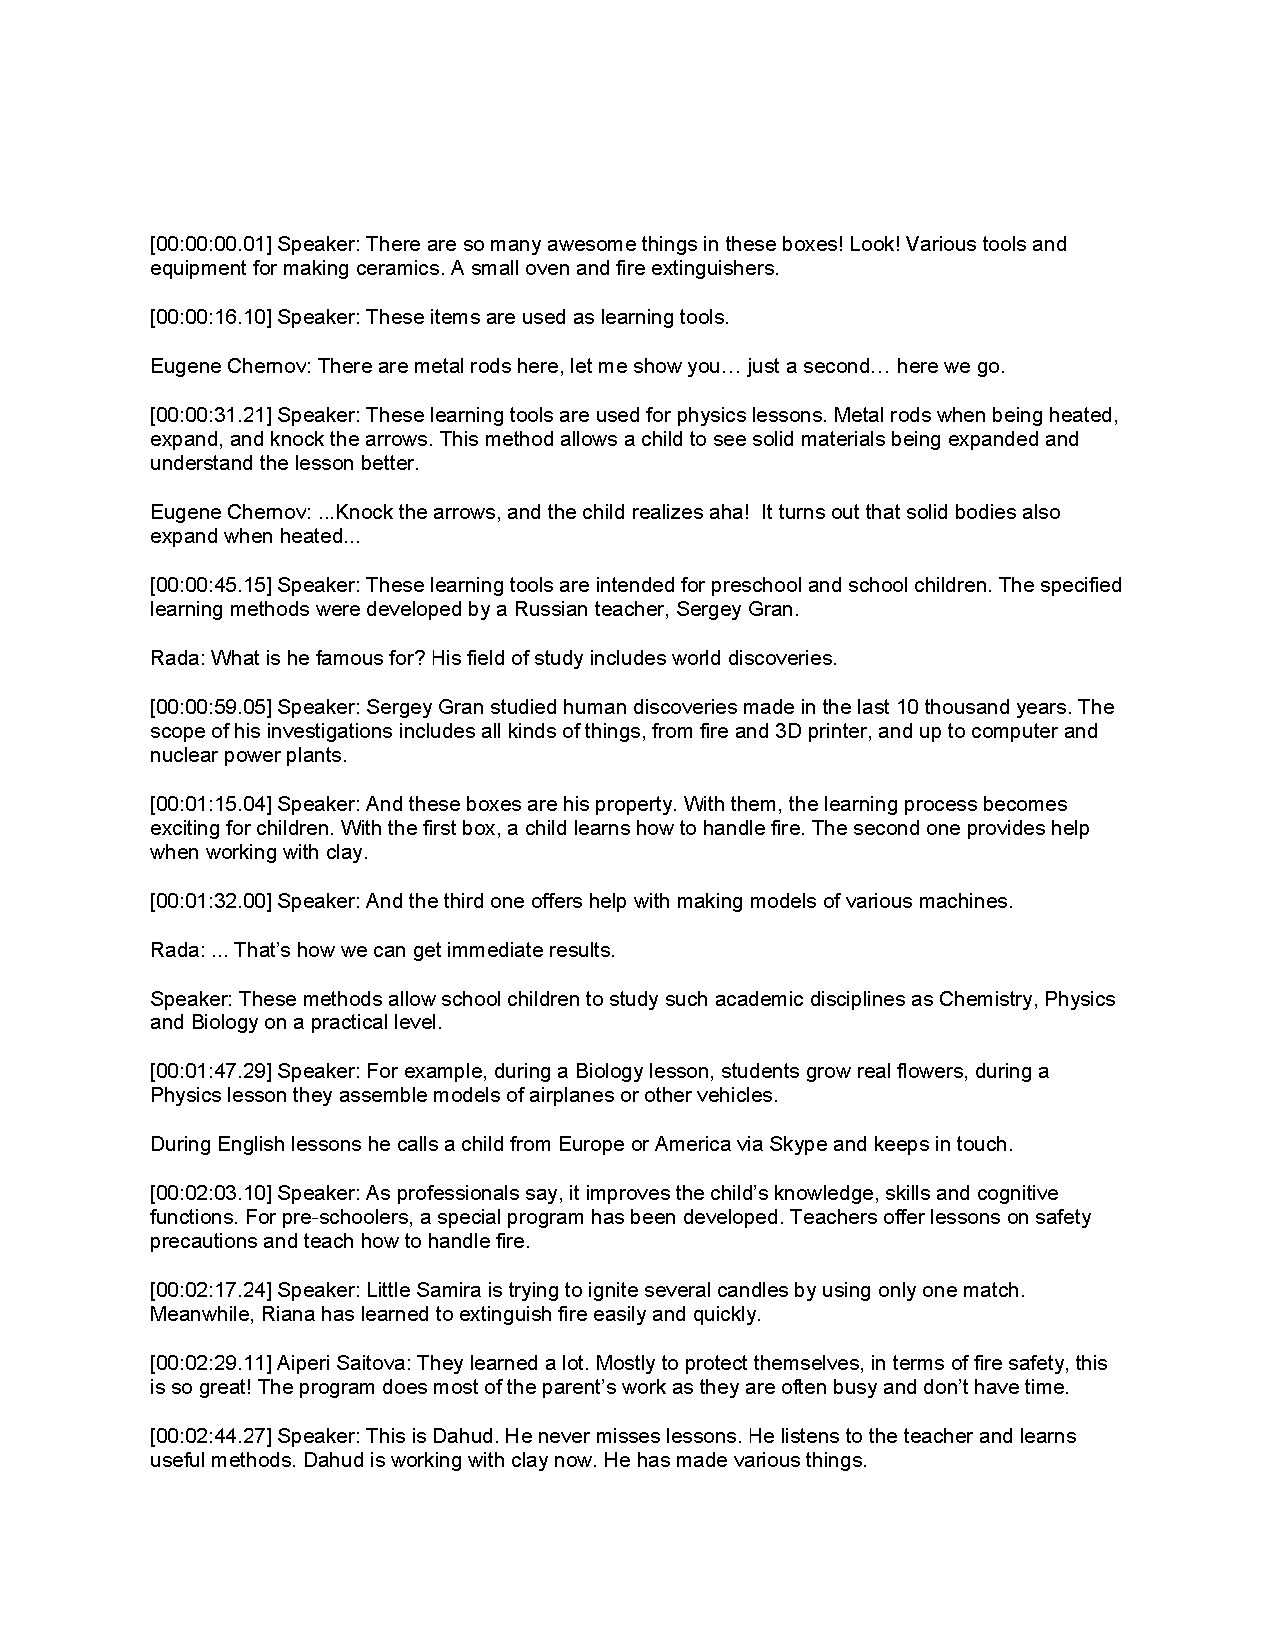
\includepdf[pages=-]{transcript_en_public}

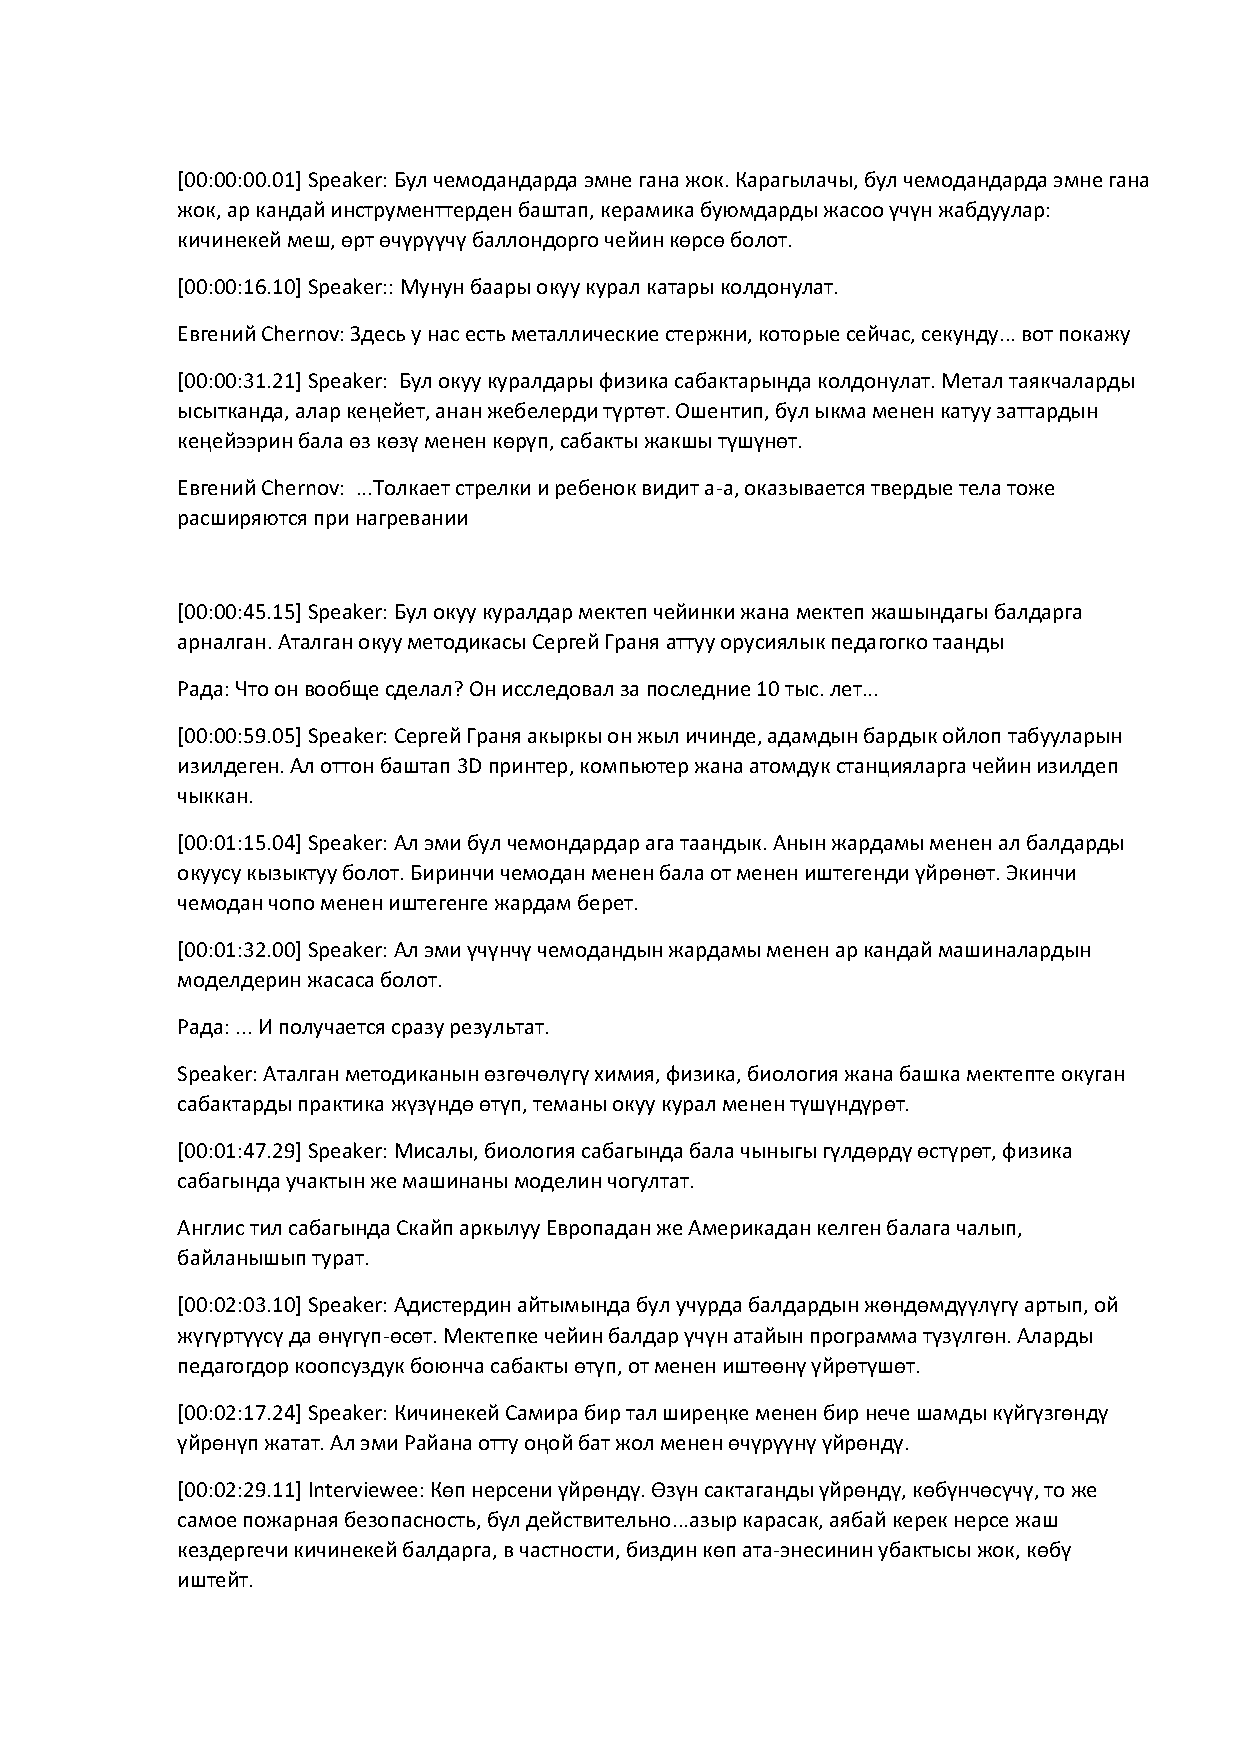
\includepdf[pages=-]{transcript}

\pagebreak
